\chapter{Évolution Différentielle}

\section{Introduction}

L'Évolution Différentielle (ED) est un algorithme évolutionnaire développée par Storn et Price \cite{Storn1995} en 1995. Il est versatile et relativement simple à implémenter et utiliser, ce qui en fait un outil essentiel dans toute boite à outils d'optimisation. Comme toutes les techniques évolutionnaires, le principe de l'évolution différentielle repose sur la génération d'une population de $N_P$ solutions (ou "vecteurs") qui permettent d'évaluer une fonction objectif à des points initiaux distribués aléatoirement dans un espace de recherche borné selon l'utilisateur. Ces points sont "perturbés" dans les générations successives de la population pour essayer de trouver des solutions extrémisant la fonction objectif. L'une des caractéristiques qui font la particularité de tout algorithme évolutionnaire est l'opération utilisée pour effectuer cette perturbation. Dans le cas de l'évolution différentielle, on perturbe une solution avec la différence de deux autres vecteurs de la population, multipliée par un facteur F, c'est l'opération dite de "mutation" comme est présenté dans la figure \ref{fig:deflowchart}. Ce nouveau vecteur subit une opération de croisement avec le vecteur initial pour produire le vecteur d'essai qui est comparé avec le vecteur de même indice dans la population. Ceci est refait jusqu'à ce que tous les vecteurs de la population soient comparés avec un vecteur d'essai (soit $N_P$ fois), créant la génération suivante. L'algorithme continue à créer de plus en plus de générations jusqu'à ce qu'un critère d'arrêt est satisfait. Souvent c'est un nombre de générations maximal ou une valeur de tolérance sur la fonction objectif.

\begin{figure}[H]
  \begin{center}
    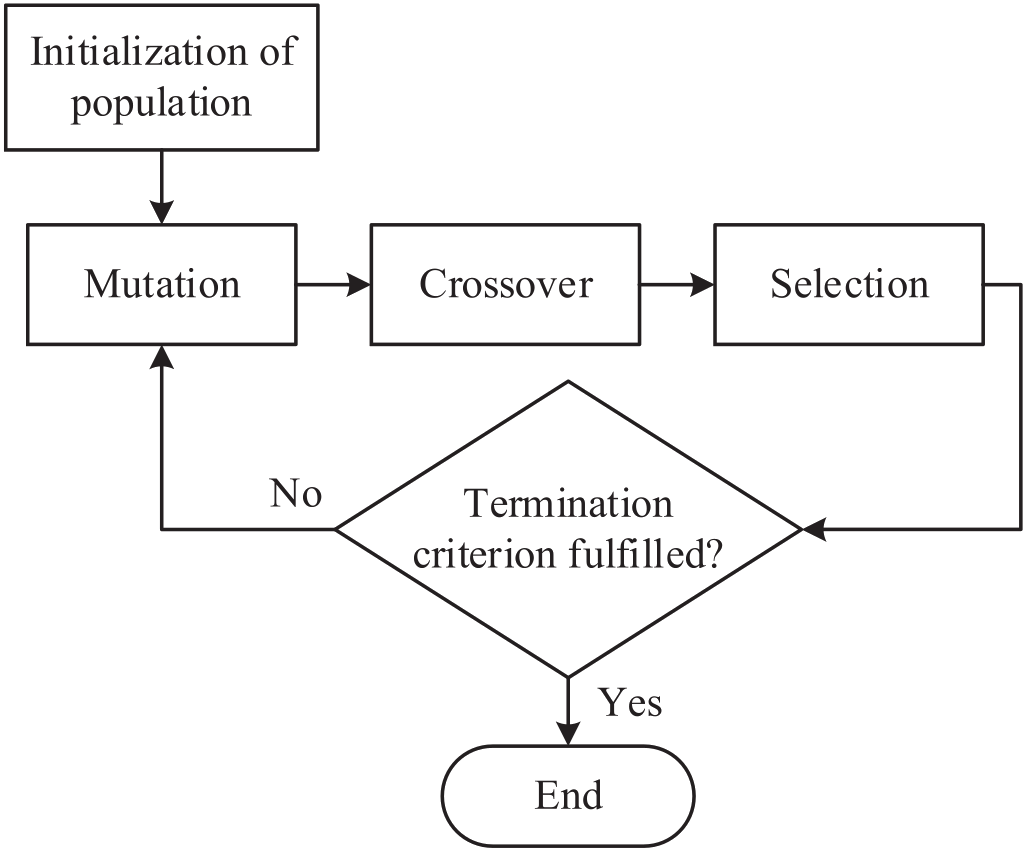
\includegraphics[width=.6\textwidth]{resources/DE.png}
    \caption{Organigramme des étapes de l'Évolution Différentielle \cite{Chin2019}}
    \label{fig:deflowchart}
  \end{center}
\end{figure}

\section{Description de l'algorithme}

\subsection{Initialisation}

La convergence des techniques d'optimisation non-linéaires est toujours conditionnée par un "bon" choix des conditions initiales. Dans le cas de l'évolution différentielle, il s'agit de l'ensemble des vecteurs constituants la population initiale. Si un vecteur solution quelconque se constitue de $D$ paramètres, notre espace de recherche est dit à $D$ dimensions, ce qui fait que notre population initiale se compose de $N_P$ vecteurs à $D$ éléments. Mais pour pouvoir effectuer l'initialisation de la population, les bornes de l'espace de recherche doivent être spécifiées. Chacun des $D$ paramètres doit avoir une borne supérieure et inférieure, ce qui fait un total de $2 \times D$ valeurs pour spécifier complètement les limites de l'espace. Reste le mécanisme utilisé pour effectivement générer les vecteurs dans cet espace borné. Pour couvrir entièrement et uniformément cet espace, il faut, pour chaque paramètre de chaque vecteur, générer aléatoirement et uniformément une valeur comprise dans la fourchette déterminée par un générateur de nombres aléatoires. En considérant que l'indice $j$ associé à un vecteur $\vec{V}$ désigne le $j-$ème paramètre, on peut accomplir ceci avec la formule \ref{eq:popinit}. 

\begin{equation}
  \label{eq:popinit}
  V_j = V_{\text{min},j} + \text{rand}[0, 1](V_{\text{max},j} - V_{\text{min},j})
\end{equation} 

On suppose avoir accès à une fonction $\text{rand}[0, 1]$, qui joue le rôle du générateur de nombres aléatoires uniformes et que $0 \leq \text{rand}[0, 1] < 1$. 
$V_{\text{min},j}$ et $V_{\text{max},j}$ sont les bornes inférieures   et supérieures du $j-$ème paramètres, respectivement. Figure \ref{fig:initpop} montre un exemple d'une population initialisée dans un espace de recherche 2 dimensionnel. Les contours sont les \textit{"isolignes"} de la fonction objectif, le minimum global doit être à l'intérieur de la fourchette spécifiée. 

\begin{figure}[H]
    \begin{tikzpicture}[>=stealth]
        \draw[help lines, color=gray!30, dashed] (0,0) grid (9.9,8.9);
        \draw[->,ultra thick] (-.5,0)--(10,0) node[right]{$V_1$};
        \draw[->,ultra thick] (0,-.5)--(0,9) node[above]{$V_2$};
        \draw[dashed] (8.2, 1) -- (0, 1)  node[left]{$V_{2, min}$};
        \draw[dashed] (8.2, 8) -- (0, 8)  node[left]{$V_{2, max}$};
        \draw[dashed] (1, 8.2) -- (1, 0) node[below]{$V_{1,min}$};
        \draw[dashed] (8, 8.2) -- (8, 0) node[below]{$V_{1,max}$};
        \draw[rotate around ={45:(4.5,4.5)}] (4.5, 4.5) ellipse (4 and 2.5);
        \draw[rotate around ={45:(4.5,4.5)}] (4.5, 4.5) ellipse (3 and 1.66);
        \draw[rotate around ={45:(4.5,4.5)}] (4.5, 4.5) ellipse (1.6 and 0.88);

        \tkzDefPoint(2.5, 3){0};
        \tkzDefPoint(2.2, 5){1};
        \tkzDefPoint(7, 6){2};
        \tkzDefPoint(5.5, 3.5){3};
        \tkzDefPoint(4, 2){4};
        \tkzDefPoint(4, 6.6){5};
        \tkzDefPoint(7, 7){6};
        \tkzDefPoint(6.5, 4){7};
        \tkzDefPoint(5.5, 7){8};
        \tkzDefPoint(4.5, 5.5){9};

        \foreach \n in {0, 1, 2, 3, 4, 5, 6, 7, 8, 9}
          \node at (\n)[circle,fill,inner sep=2pt]{};
        \foreach \n in {0,1,2,3,4,5,6,7,8,9}
          \tkzLabelPoint[above](\n){$\n$};
    \end{tikzpicture}
    \caption{Exemple d'une population initialisée dans un espace de recherche à deux dimensions. Dans ce cas $D = 2$, $N_P = 10$ et l'indice de génération $g = 0$ puisqu'il s'agit de la population initiale}
    \label{fig:initpop}
\end{figure}
\clearpage

\subsection{Mutation}
\nomenclature[1vbase]{$\vec{V}_{base}$}{Vecteur de base}
\nomenclature[1vmut]{$\vec{M}_{i}$}{Vecteur mutant}
\nomenclature[1vessai]{$\vec{T}_{i}$}{Vecteur d'essai}

Après l'initialisation de la population, l'ED modifie, croise et recombine la population pour produire des vecteurs d'essai (un nombre $N_P$ de ces vecteurs) qui seront comparés avec les vecteurs cibles qui leurs correspondent dans la population. La \textit{Mutation} dans l'ED est en fait une "mutation différentielle". Elle consiste à ajouter la différence de deux vecteurs choisis aléatoirement de la population, multipliée par un facteur de pondération ou "Facteur de Mutation", à un troisième vecteur de base distinct. Cette opération produit un vecteur mutant $M$ selon l'équation \ref{eq:mutant}. L'indice $i$ indique le $i$-ème vecteur de la population, et $gen$ la génération où l'on est. 
Il n'y a pas de limite dure sur le Facteur de Mutation $F$, mais les valeurs supérieures à $1$ sont rarement considérées. Dans notre cas, on considère que $F \in [0, 1]$. Il existe plusieurs stratégies pour choisir le $\vec{V}_{base}$, le seul prérequis étant qu'il soit distinct du vecteur cible. Dans ce travail nous utiliserons exclusivement le choix du vecteur ayant la meilleure qualité ou valeur de "fitness" calculée par la fonction objectif. Les vecteurs de la différence $\vec{V}_{r1,gen}$ et $V_{r2,gen}$ sont choisis aléatoirement de la population pour chaque vecteur mutant et ne doivent qu'être distincts l'un de l'autre et des vecteurs cible $\vec{V}_{i, gen}$ et de base $\vec{V}_{base, gen}$.

\begin{equation}
  \label{eq:mutant}
  \vec{M}_{i,gen} = \vec{V}_{base,gen} + F (\vec{V}_{r1,gen} - \vec{V}_{r2,gen})  
\end{equation}

\begin{figure}[H]
    \begin{tikzpicture}[>=stealth]
        \draw[help lines, color=gray!30, dashed] (0,0) grid (9.9,8.9);
        \draw[->,ultra thick] (-.5,0)--(10,0) node[right]{$V_1$};
        \draw[->,ultra thick] (0,-.5)--(0,9) node[above]{$V_2$};
        
        \tkzDefPoint(6, 4){0};
        \tkzDefPoint(8, 3){1};
        \tkzDefPoint(6, 6){2};
        \tkzDefPoint(6- 1.5, 4 + 2.25){3};
        
        \node at (0)[circle,fill,inner sep=1.2pt]{};
        \tkzLabelPoint[left](0){\smaller $\vec{V}_{base,gen}$};
        \node at (1)[circle,fill,inner sep=1.2pt]{};
        \tkzLabelPoint[right](1){\smaller $\vec{V}_{r2,gen}$};
        \node at (2)[circle,fill,inner sep=1.2pt]{};
        \tkzLabelPoint[right](2){\smaller $\vec{V}_{r1,gen}$};
        \node at (3)[circle,fill,color=blue,inner sep=1.2pt]{};
        \tkzLabelPoint[above](3){\color{blue}{\smaller $\vec{M}_{i,gen} = \vec{V}_{base,gen} + F (\vec{V}_{r1,gen} - \vec{V}_{r2,gen})$}};
        
        \draw[->, thick] (1) -- (6.5, 5.25) node[midway, right]{\smaller $F (\vec{V}_{r1,gen} - \vec{V}_{r2,gen})$};
        
        \draw[dashed] (1) -- (2);
        \draw[dashed] (1) -- (0);
        \draw[dashed] (6.5,5.25) -- (3);
        \draw[dashed] (0) -- (3);
        
        \draw[draw=blue, ->, ultra thick] (0, 0) -- (3);
        
    \end{tikzpicture}
    \caption{L'opération de mutation différentielle ajoute $F (\vec{V}_{r1,gen} - \vec{V}_{r2,gen})$ au vecteur de base $\vec{V}_{base,gen}$ pour produire un mutant $\vec{M}_{i,gen}$}
    \label{fig:mutant2}
\end{figure}

\subsection{Croisement}
La opération de mutation est suivie d'un croisement ou \textit{recombinaison discrète}. Elle consiste à construire le vecteur d'essai $\vec{T}_{i,gen}$ à partir des éléments (i.e. paramètres) de deux vecteurs différents selon une probabilité spécifiée. Chaque élément $j$ du vecteur d'essai est choisi selon la formule \ref{eq:cross}.


\begin{equation}
  \label{eq:cross}
  T_{j,i,gen} =
  \begin{cases}
    M_{j,i,gen} & \text{si}\ \text{rand}[0, 1] \leq CR\ \text{ou}\ j = j_{rand}\\
    V_{j,i,gen} & \text{sinon}
  \end{cases}
\end{equation}

$CR \in [0,1]$ détermine la probabilité que le paramètre provienne du vecteur mutant tant que $\text{rand}[0, 1]$ est effectivement un générateur aléatoire uniforme. Le taux de croisement $CR$ est l'un des paramètres spécifiés par l'utilisateur au début. Un nombre aléatoire $j_{rand}$ est aussi choisi tel que $0 \leq j_{rand} < D$ pour s'assurer que le nouveau vecteur d'essai ne duplique pas complètement le vecteur cible $\vec{V}_{i,gen}$.

\subsection{Sélection}
Si le vecteur d'essai $\vec{T}_{i,gen}$ est évalué à une valeur inférieure par la fonction objectif $f$ au vecteur cible $\vec{V}_{i,gen}$, il le remplace dans la génération suivante (i.e. $gen + 1$). Sinon le vecteur cible survit à la sélection et retient sa place dans la génération suivante (équation \ref{eq:selection}).
Quand la nouvelle population est complète, le processus de mutation, croisement et sélection est renouvelé jusqu'à ce qu'un critère d'arrêt est vérifié (e.g. un nombre maximal de générations $gen_{max}$)

\begin{equation}
  \label{eq:selection}
  \vec{V}_{i, gen + 1} =
  \begin{cases}
    \vec{T}_{i,gen} & \text{si}\ f(\vec{T}_{i,gen}) \leq f(\vec{V}_{i,gen})\\
    \vec{V}_{i,gen} & \text{sinon}
  \end{cases}
\end{equation}

\section{Remarques}
On vient de citer toutes les étapes de l'ED "classique" comme elle a été présenté par Storn et Price 2005 \cite{Price2005}. Cependant il existe plusieurs variations ou "stratégies" de l'ED selon la manière avec laquelle on choisi le vecteur de base avant la mutation, le nombre de différences pondérées ajoutées et la méthode de croisement. Nous avons opté à choisir le vecteur à meilleure valeur de fitness comme vecteur de base, auquel on ajoute une seule différence de vecteurs pondérée par $F$, et finalement un croisement binomial. Le mot technique pour cette stratégie est "DE/best/1/bin" dont une demonstration en pseudocode est dans l'algorithme \ref{alg:debestbin} dans la section suivante.

Il faut aussi noter que cet algorithme comme il est, n'est contraint nul part à ne générer que des solutions comprises dans les limites initiales de l'espace de recherche. Ceci présente en fait un avantage de l'ED puisque ça permet d'explorer les zones au-delà des limites de la population initiale pour potentiellement trouver un minimum global qu'on est pas toujours assurés qu'il soit dans la zone initiale. Cependant, on peut tomber sur des solutions non "physiques" et qui ne présentent aucun intérêt pour notre application. Storn et Price citent plusieurs techniques pour résoudre ce problème, mais dans notre cas on effectue un test sur chaque vecteur mutant. Si un de ses paramètres se retrouve à l'extérieur des limites spécifiées de l'espace de recherche, on le pénalise en imposant une valeur de fitness assez large pour éliminer les chances que ce vecteur pourra survivre vers la génération suivante.

Dans notre application de l'ED sur le problème d'identification des paramètres de modèles à diodes, nous prenons l'approche d'un problème d'optimisation. En effet, un vecteur solution se constitue de tous les paramètres nécessaires pour une description complète du modèle équivalent, c'est-à-dire un espace de recherche à $D = 5$ dimensions dans le cas du modèle simple diode ($R_P$), et à D = 7 dimensions dans le cas du modèle double diode. La fonction objectif à minimiser devrait être une mesure de la différence entre la courbe I-V du modèle et celle de la cellule experimentale. La méthode la plus répandue pour quantifier cette différence est la racine de l'erreur quadratique moyenne ou \textit{Root Mean Squared Error}. L'erreur d'un vecteur $\vec{V}_{sol}$ est donnée par l'équation \ref{eq:rmse} où l'indice $i$ indique un point dans la courbe caractéristique I-V.

\begin{equation}
  \label{eq:rmse}
  f(\vec{V}_{sol}) = RMSE = \sqrt{\frac{1}{N} \sum_{i = 1}^{N} (I_{i,exp} - I_{i, cal}(\vec{V}_{sol}))^2 }
\end{equation}

\section{Pseudo-code}
Une implémentation de l'Évolution Différentielle en pseudo-code est la suivante:

\begin{algorithm}[H]
  $F \gets$ Facteur de mutation\;
  $CR \gets$ Taux de croisement\;
  $N_P \gets$ Taille de la population\;
  $gen_{max} \gets$ Nombre de générations\;
  $D \gets $ Nombre de paramètres\;
  
  $gen = 0$\;
  $\text{Initialize population\ } P_0 = [V_0, V_1, .., V_{N_P}]$\;
  \For{$i = 0 \text{\ to\ } N_P$}{
      $V_{min} = [V_{1,min}, V_{2,min}, .., V_{D,min}]$\;
      $V_{max} = [V_{1,max}, V_{2,max}, .., V_{D,max}]$\;
      $V_{i} = V_{min} + \text{rand}[0, 1] (V_{max} - V_{min})$\;
  }
  \While{$gen < gen_{max}$}{
    \For{$j = 0$\ to\ $N_P$}{
      $V_{j,gen} = [V_{1,j,gen}, V_{2,j,gen}, .., V_{D,j,gen}]$\;
      Choisir le vecteur de base et deux vecteurs aléatoires $V_{r1}\ \text{et}\ V_{r2} \in P_{gen}$\;
      $V_{base} = V \in P_{gen} \mid \forall (K \in P_{gen}), \quad f(V) \leq f(K)$\;
      Mutation :\\
      $M_{j,gen} = V_{base} + F (V_{r1} - V_{r2})  $\;
      Croisement : \\
      $T_{j,gen} = [T_{1,j,gen}, T_{2,j,gen}, .., T_{D,j,gen}]$\;
      \eIf{rand$[0, 1] < CR\ $ or\ $j = j_{rand}$}{
        $T_{i,j,gen} = M_{i,j,gen}$\;
      }{
        $T_{i,j,gen} = V_{i,j,gen}$\;
      }
      Selection :\\
      \eIf{$f(T_{j,gen}) < f(V_{j,gen})$}{
        $V_{j,gen + 1} = T_{j, gen}$\;
      }{
      $V_{j,gen + 1} = V_{j, gen}$\;
      }
    }
    $gen = gen + 1$\;
  }
  \caption{Stratégie DE/best/1/bin}
  \label{alg:debestbin}
\end{algorithm}

%\section{Métaheuristique}

\section{Conclusion}
Maintenant que nous avons décrit l'évolution différentielle tel qu'elle a été décrite par Storn et Price, nous avons opté à utiliser la stratégie DE/best/1/bin et l'erreur quadratique moyenne comme fonction objectif. Dans ce qui suit, il va falloir rendre l'évolution différentielle compatible avec les modèles à diodes cité dans le chapitre 1. Pratiquement, il faudrait concevoir une méthode pour retrouver la caractéristique IV associée à chaque vecteur solution pour pouvoir calculer son erreur quadratique moyenne par rapport aux données expérimentales. Ceci va ensuite permettre à l'évolution différentielle d'effectuer ses opérations de sélection selon la fonction objectif.
